\documentclass[tikz,border=6pt]{standalone}
\usepackage{amsmath}
\usetikzlibrary{arrows.meta,positioning,fit,backgrounds}
\begin{document}
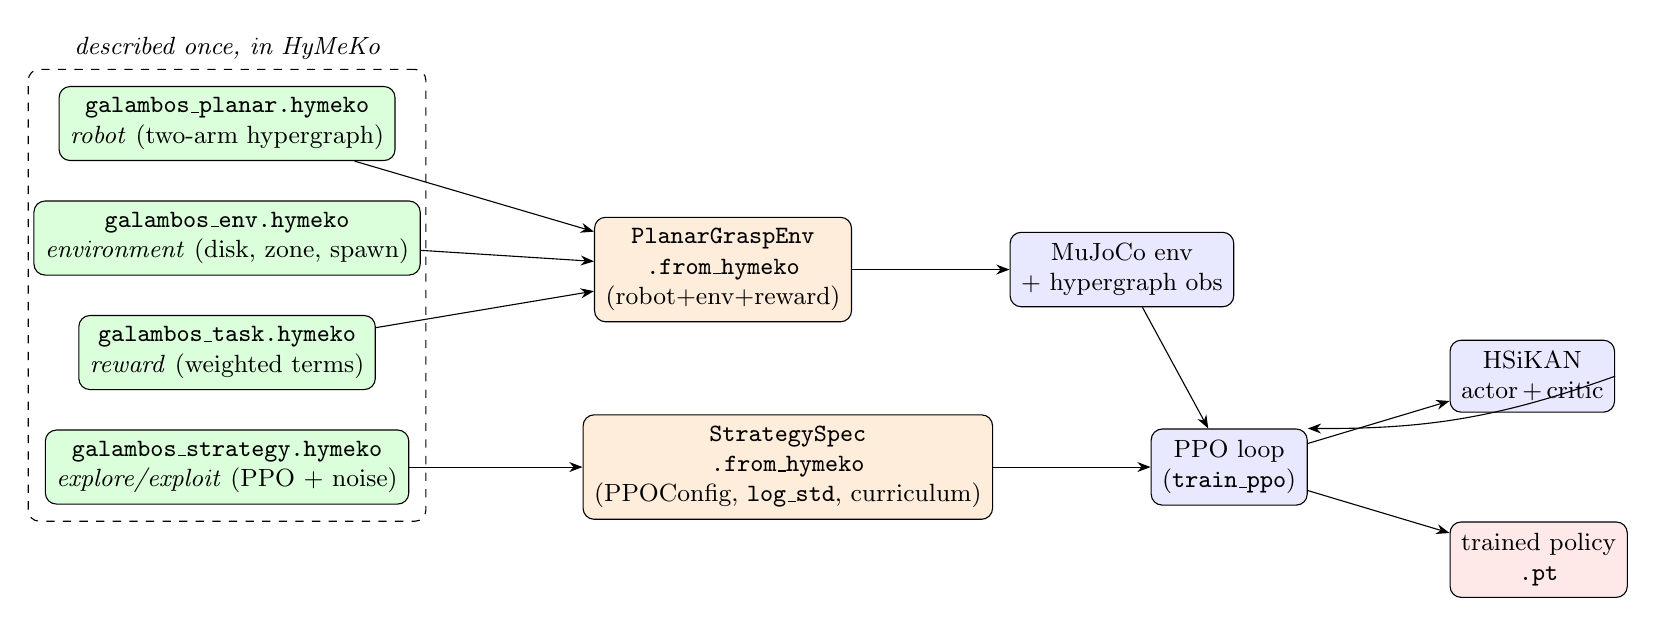
\begin{tikzpicture}[
  font=\small, >={Stealth[]}, node distance=5mm and 16mm,
  hy/.style={draw, rounded corners, fill=green!14, align=center, inner sep=4pt, minimum height=8mm},
  rd/.style={draw, rounded corners, fill=orange!14, align=center, inner sep=4pt, minimum height=8mm},
  obj/.style={draw, rounded corners, fill=blue!9,  align=center, inner sep=4pt, minimum height=8mm},
  res/.style={draw, rounded corners, fill=red!9,   align=center, inner sep=4pt, minimum height=8mm}]

  % --- the four .hymeko sources (everything as data) ---
  \node[hy] (robot)  {\texttt{galambos\_planar.hymeko}\\\textit{robot} (two-arm hypergraph)};
  \node[hy, below=of robot] (env) {\texttt{galambos\_env.hymeko}\\\textit{environment} (disk, zone, spawn)};
  \node[hy, below=of env]  (task) {\texttt{galambos\_task.hymeko}\\\textit{reward} (weighted terms)};
  \node[hy, below=of task] (strat){\texttt{galambos\_strategy.hymeko}\\\textit{explore/exploit} (PPO + noise)};

  % --- readers / composition ---
  \node[rd, right=22mm of env, yshift=-4mm] (fh) {\texttt{PlanarGraspEnv}\\\texttt{.from\_hymeko}\\(robot+env+reward)};
  \node[rd, right=22mm of strat] (ss) {\texttt{StrategySpec}\\\texttt{.from\_hymeko}\\(PPOConfig, \texttt{log\_std}, curriculum)};

  % --- runtime objects ---
  \node[obj, right=20mm of fh] (envobj) {MuJoCo env\\+ hypergraph obs};
  \node[obj, right=20mm of ss] (ppo) {PPO loop\\(\texttt{train\_ppo})};

  % --- policy + output ---
  \node[obj, above right=2mm and 18mm of ppo] (policy) {HSiKAN\\actor\,+\,critic};
  \node[res, below right=2mm and 18mm of ppo] (ckpt) {trained policy\\\texttt{.pt}};

  \draw[->] (robot) -- (fh); \draw[->] (env) -- (fh); \draw[->] (task) -- (fh);
  \draw[->] (strat) -- (ss);
  \draw[->] (fh) -- (envobj);
  \draw[->] (ss) -- (ppo);
  \draw[->] (envobj) -- (ppo);
  \draw[->] (ppo) -- (policy);
  \draw[->] (policy.east) to[bend left=10] (ppo.north east);
  \draw[->] (ppo) -- (ckpt);

  \begin{scope}[on background layer]
    \node[draw, dashed, rounded corners, fit=(robot)(strat), inner sep=6pt,
          label={[font=\small\itshape]above:described once, in HyMeKo}] {};
  \end{scope}
\end{tikzpicture}
\end{document}
